\documentclass[seminar]{fer}

\usepackage[authoryear]{natbib}
\title{Detekcija pješaka u urbanim okruženjima korišenjem značajki temeljenih na teksturi i boji}
\author{Iva Miholić, Gustav Matula, Kristijan Franković, Tomislav Kiš}

\begin{document}
\maketitle

\chapter{Detekcija pješaka u urbanim okruženjima}
\section{Opis zadatka i postojećih rješenja}
Detekcija pješaka u urbanim okruženjima problem je povezan sa automobilskom industrijom, sigurnošću u prometu, sigurnosnim nadziranjem i robotikom. Rješava se kao detekcija objekta u okviru područja računalnog vida. Ovaj projektni zadatak obuhvaća izgradnju detektora pješaka na fotografijama iz urbanih okruženja korištenjem značajki temeljenih na teksturi i boji.

Pregled najznačajnijih rješenja ovog problema dan je u \cite{BenensonOHS14}. Prvi značajniji napredak u detekciji pješaka bila je primjena \emph{VJ} detektora objekata \cite{VJ} na ovaj problem. Detektori temeljeni na histogramu usmjerenih gradijenata \engl{Histogram of Oriented Gradients, HOG} \cite{HOG}  uz linearni ili nelinearni skup potpornih vektora, postigli su značajne rezultate, posebice u kombinaciji sa drugim značajkama temeljenih na svojstvima boje, tekstura i oblika. Više o HOG pristupu bit će riječi u sljedećim poglavljima jer ćemo ga koristiti kao kostur našeg prostora značajki.

Od ostalih rezultata, potrebno je izdvojiti postupke temeljene na modelu rastavljivih dijelova  \engl{Deformable Part Models, DPM} u kojem se detekcija dijelova tijela sažima u detekciju cijelog pješaka te nelinearne postupke učenja temeljenih na neuronskim mrežama i stabalima odluke \cite{BenensonOHS14}. Takvi složeniji postupci uspoređeni su sa linearnim SVM-om uz HOG i druge značajke nisu dali značajno bolji rezultat upućujući na korektnost naše odluke o arhitekturi detektora.

Pristup na koji ćemo se fokusirati koristi metodu skalabilnog kliznog prozora. Unutar prozora na fotografiji određuju se značajke te se skup piksela unutar prozora binarno klasificira kao fotografija pješaka. Prozor zatim "putuje" po fotografiji testirajući druge skupove piksela te se može dodatno skalirati nakon čega se ponavlja isti postupak. Primjer klasificirane fotografije ovakvim postupkom vidljiv je na slici \ref{primjer_klasifikacije}. Problem takvog pristupa je ignoriranje konteksta oko okvira koji se promatra što se uspješno rješava uvođenjem novih značajki, odnosno novih informacija o prozoru u sustav.
\begin{figure}
\center
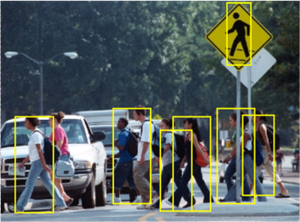
\includegraphics[scale=0.7]{img/crossing.png}
\caption{Fotografija koja je klasificirana detektorom pješaka metodom kliznog prozora. Žuti okviri prikazuju okvire onih prozora koji su klasificirani kao prikaz pješaka.}
\label{primjer_klasifikacije}
\end{figure}

Do sada su najviše korištene značajke temeljene na informaciji o bridovima, boji, teksturi loklalnim oblicima te svojstvima gradijenta i kovarijance. Dodavanje novih značajki pokazao se kao vrlo uspješan način poboljšanja rada detektora pješaka, no proširenje prostora značajki može biti problematično za klasične algoritme učenja što se rješava redukcijom prostora značajki metodom Fisherove diskriminantne analize ili postupkom parcijalnih najmanjih kvadrata \engl{Partial Least Squares, PLS} \cite{Schwartz_humandetection}. 

\chapter{Baza podataka za treniranje i verifikaciju rješenja}

Za treniranje i verifikaciju rješenja koristit ćemo skup podataka INRIA \cite{DT05}. To je skup fotografija urbanog okruženja u boji i pripadnih anotacija. Za svaku fotografiju zabilježen je skup graničnih prozora \engl{bounding window} unutar kojih se nalaze prikazi uspravnih osoba.

INRIA se do sada često koristio za trening detektora zbog raznolikosti pozadinskih okruženja osoba na slikama i točnosti anotacija \cite{BenensonOHS14}. Za razliku od ostalih javno dostupnih baza podataka za detekciju pješaka, ove fotografije nisu dobivene iz videa te su relativno visoke kvalitete i fotografirane su iz različitih točaka gledišta. U drugim bazama podataka, pješaci su većinom konecentrirani u centralnoj horizontali fotografije jer je ista dobivena iz vozačeve perspektive.

Baza se sastoji od podskupa za trening i podskupa za evaluaciju. U podskupu za trening označena su $1208$ pješaka u $614$ od $1832$ fotografije. U podskupu za testiranje označeno je $566$ pješaka u $453$ od $741$ fotografije \cite{Dollar:2012:PDE:2197081.2197275}

\chapter{Idejno rješenje i prikaz arhitekture sustava računalnog vida}

\section{Pregled značajki temeljenih na teksturi i boji}

Značajke temeljene na teksturi i boji obično se koriste kao nadopuna značajkama fokusiranim na bridove, za koju ćemo koristiti popularnu HOG
metodu Dalal i Triggsa \cite{HOG}. Njihova se metoda pokazala dobrom na više baza, ali promatranjem isključivo gradijenata potencijalno odbacujemo
korisne izvore informacija, što vodi lažnoj pozitivnoj klasifikaciji.

Primjerice tekstura nam dosta pomaže kod prepoznavanja odjeće, ali i pozadine, a boja kod prepoznavanja boje kože.


Pretpostavljamo (slično kao u \cite{Schwartz}) da je detekcijski prozor podijeljen na preklapajuće blokove u iz kojih se zatim ekstrahiraju značajke.

\subsection{Značajke temeljene na teksturi}

Vjerojatno najpoznatija metoda ekstrakcije značajki koje opisuju teksturu potječe iz Haralickovog rada \cite{Haralick} još iz 1979. Za opis teksture koristi takozvanu \emph{co-occurrence} matricu, iz koje se zatim računaju same značajke, kao što su npr. korelacija, srednje vrijednosti i razne mjere entropije.


Osnovna ideja iza matrice jest određivanje vjerojatnosti susjedstva svih parova intenziteta. Tako primjerice horizontalna matrica $H$ kao element
$h_{i,j}$ sadrži vjerojatnost da je nasumični par horizontalno susjednih piksela ima intenzitete redom $i$ i $j$. Matrica se tipično računa za horizontalni, vertikalni, te oba dijagonalna smjera. Još jedan parametar koji se može koristiti jest udaljenost $d$, pa tako matrica $V^{(d)}$ uzima u obzir 
parove koji su vertikalno susjedni na udaljenosti $d$.


Tako dobivena matrica tada se promatra kao matrica zajedničke distribucije vjerojatnosti $p(i, j)$, te iz nje računamo značajke. Tipični
primjeri značajki koje Haralick navodi u svome radu su primjerice:

\begin{itemize}
  \item
  Varijanca: $$\sum_{i}\sum_{j}(i - \mu)^2p(i, j)$$
  \item
  Korelacija: $$\frac{\sum_{i}\sum_{j}(ij)p(i,j) - \mu_{x}\mu_{y}}{\sigma_{x}\sigma_{y}}$$
  \item
  Entropija: $$-\sum_{i}\sum_{j}p(i, j)\log(p(i, j))$$
\end{itemize}

\subsection{Značajke temeljene na boji}


U \cite{Schwartz} se za iskorištavanje informacije sadržane u boji koristi jednostavno proširenje HOG histograma. Za početak, HOG histogram se gradi tako da se za
svaki piksel uzima gradijent po boji s najvećom normom, dakle promatramo koja boja se najviše mijenja. Zatim se formira trostupčani histogram frekvencija svake od tri boje za trenutni prozor detekcije. Tako uz histogram gradijenata promatramo i histogram boja.


\subsection{Redukcija dimenzije}


Velika dimenzija prostora značajki koju dobivamo promatrajući, uz gradijente, teksturu i boju, predstavlja problem za klasične metode strojnog učenja
za treniranje klasifikatore. Zbog podjele prozora detekcije u blokove, značajke se ekstrahiraju iz susjednih blokova, što neizbježno vodi do
sličnih značajki bliskih blokova i samim time do kolinearnosti. Zbog toga ima smisla iskoristiti nekakvu tehniku redukcije dimenzije, kao što su
PCA (\emph{Principal Component Analysis}) ili FDA (\emph{Fisher Discriminant Analysis}). \cite{Schwartz} koristi PLS (\emph{Partial Least Squares}), inače 
regresijsku metodu, praktičnu i za redukciju dimenzije skupa značajki. 

Nakon redukcije dimenzije za treniranje klasifikatora možemo koristiti metode tipa SVM (\emph{Support Vector Machine}), koje bi na prostoru s 
previše dimenzija bile neupotrebljive.


\section{Plan arhitekture sustava računalnog vida}

Sustav će se kao i obično sastojati od dvije osnovne komponente: treniranja i primjene.

\subsection{Treniranje klasifikatora}

\begin{figure}[h!]
\center
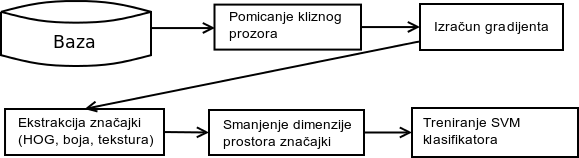
\includegraphics[scale=0.7]{img/treniranje.png}
\caption{Dijagram treniranja SVM klasifikatora}
\label{primjer_klasifikacije}
\end{figure}

Treniranje se sastoji od nekoliko koraka koji su okvirno prikazani na slici.1. 
Za svaku sliku iz baze računaju se gradijenti (horizontalni i vertikalni smjer). Zatim po slici pomičemo
klizni prozor, dijelimo ga na preklapajuće blokove i za svaki blok računamo histogram gradijenata i histogram boja. Prozor potom ponovno dijelimo
na blokove (ne nužno istih dimenzija kao u prethodnom koraku), te računamo \emph{co-occurrence} matricu, iz koje dobivamo značajke koje opisuju
teksturu. U sljedećem koraku reduciramo dimenziju prostora značajki. Konačno, na tako pojednostavljenim primjerima treniramo SVM.


\subsection{Primjena klasifikatora}


Slično kao kod treniranja promatramo klizni prozor i za njega računamo značajke, kojima zatim reduciramo dimenziju te ih dajemo kao input
klasifikatoru. U koliko klasifikator procijeni da se radi o pješaku, dojavljujemo poziciju trenutnog kliznog prozora



\bibliographystyle{plain}
\bibliography{bibliografija}
\end{document}
